\section{Introduction}

Time-series representation learning has advanced on top of predictive objectives --- contrastive prediction of the future \cite{oord2018}, and more recently prediction of latent representations rather than reconstruction of the raw signal \cite{lecun2022, assran2023}. A single series, however, mixes factors acting on different timescales, which makes the embedding hard to interpret. Work that pulls them apart has succeeded mainly at separating static factors, those constant over an entire sequence \cite{hsu2017, li2018}, because invariance is itself a training signal that can be written into the objective. For factors that change slowly without being constant, no such definition is available.

\begin{figure}[!tbp]
\centering
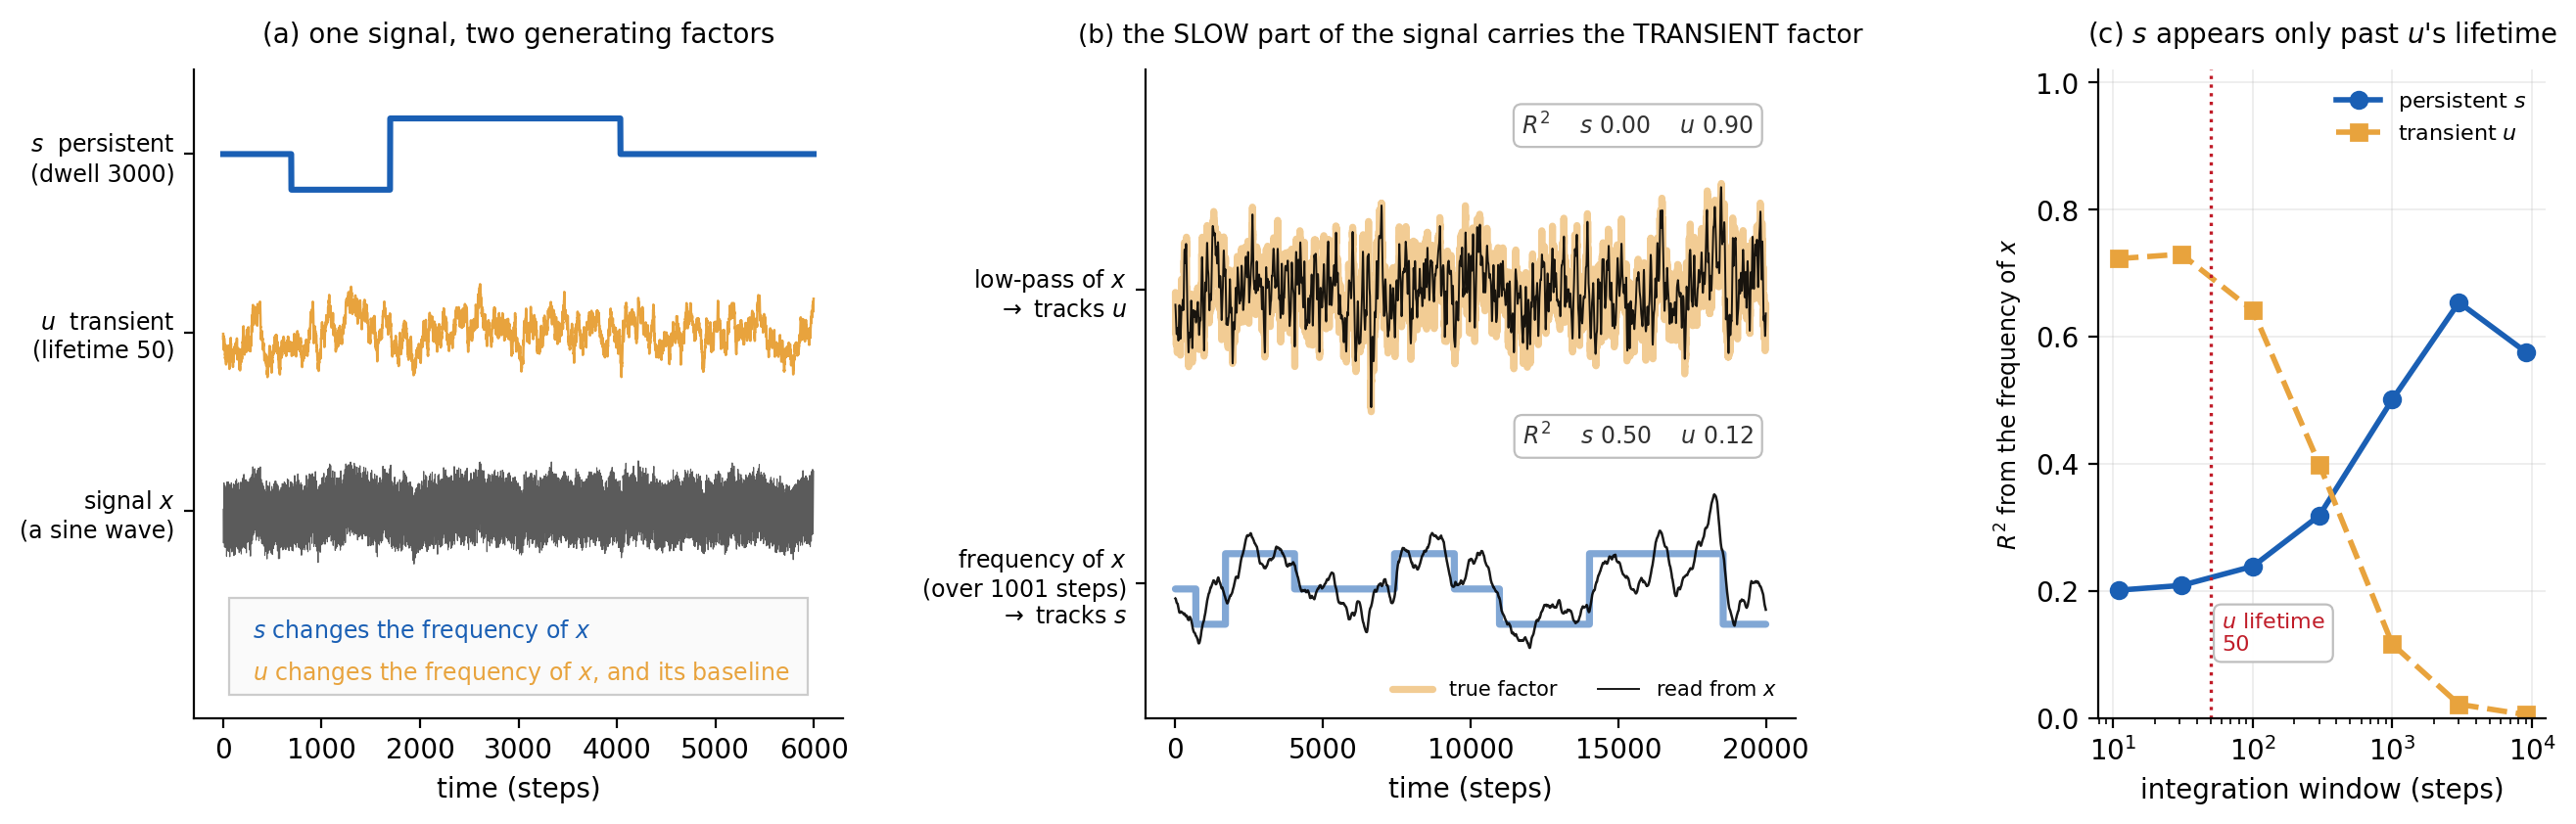
\includegraphics[width=\textwidth]{figs/fig_persistence.png}
\caption{\textbf{Spectral slowness is not factor persistence.} One synthetic series (400,000 steps, a single seed): the persistent factor $s$ switches every 3,000 steps among three frequencies 3\% apart, and the transient factor $u$ is an Ornstein--Uhlenbeck process of lifetime 50. Autocorrelation half-lives are 1,859 and 51 steps, so the two timescales are well separated. \textbf{(a)} The two factors and the signal they generate. $s$ changes only the frequency of $x$; $u$ changes its frequency and its baseline. \textbf{(b)} Reading the slow part of $x$ recovers the transient factor rather than the persistent one ($R^2$ 0.90 against 0.00), while reading the frequency of $x$ over a 1,001-step window recovers the persistent one ($R^2$ 0.50). \textbf{(c)} $R^2$ for both factors against the width of that window. The persistent factor appears only once the window is tens of times $u$'s lifetime, and falls off again when the window grows wide enough to blur $s$ itself.}
\label{fig:persistence}
\end{figure}

Separating what is ``slow'' from what is ``fast'' can mean two different things. One is separating the \emph{signal} --- decomposing the observed waveform into a trend and a fluctuation, for which long-established tools exist \cite{cleveland1990, huang1998}. The other is separating the \emph{factors} that generated the signal, the lineage of latent-factor identification from temporal structure \cite{hyvarinen2016}. This work is concerned with the factor side --- a patient's diagnosis, or the fact that a person is walking. The two readings are often treated as the same, yet they need not agree.

They can diverge in only one direction. We fix the term: a factor is \emph{persistent} if it still contributes to prediction $\Delta$ steps ahead. Under this definition the slow part of the signal is necessarily persistent, since a component confined to low frequencies has slowly decaying autocorrelation \cite{khinchin1934}, and remaining autocorrelation is a contribution to prediction at distant horizons. The converse fails: low-pass filtering is linear in the signal, whereas a factor may ride on nonlinear statistics such as frequency or variance. Fig.~\ref{fig:persistence} shows such a case on controlled data: when the persistent factor sets the frequency of the oscillation, reading only the slowly varying part of the signal recovers the transient factor ($R^2 = 0.90$) and not the persistent one ($R^2 < 10^{-5}$).

The two readings are still connected. While a factor persists, the statistics of the signal are fixed: during walking the acceleration waveform oscillates rapidly, but its variance and spectral shape stay constant. What changes slowly is not the signal but its statistics, and those appear only through some function of the signal. In Fig.~\ref{fig:persistence} that function is the oscillation frequency, read over a wide window (Fig.~\ref{fig:persistence}b); with a narrow window the reading is mostly the transient factor and turns over toward the persistent one only once the window is tens of times the transient lifetime (Fig.~\ref{fig:persistence}c).

Which band a factor appears in therefore constrains its persistence in one direction only: the slow band implies persistence, not the converse. This is an \emph{existence} claim --- such factors can exist; how often they arise in real data this paper does not answer. Our selection criterion is persistence. In our synthetic data the persistent factor is carried inside the oscillation, the fastest-changing part of the signal, while the transient factor enters as a slower additive term.

Persistence is controlled by a variable prediction-based learning already has: the horizon $\Delta$. Setting $\Delta$ farther out makes only long-persisting factors useful \cite{bialek2001, creutzig2008}. We gate that horizon and propose HGLP, which forces prediction at distant horizons to use only a designated block of coordinates. The target state is shown in Fig.~\ref{fig:concept}: an ordinary embedding mixes both factors in every coordinate, whereas we require that a nameable 16 dimensions (the $\zslow$ block) must carry the persistent factor with the transient factor emptied out of it. The latent space is rotation-symmetric, so the persistent factor can be read out of any 16 dimensions; our claim is therefore not that ``the persistent factor gathers in $\zslow$ and is absent elsewhere,'' but that ``the transient factor is emptied out of $\zslow$.'' The remaining block ($\zmix$) is unconstrained and holds both factors.

\begin{figure}[!tbp]
\centering
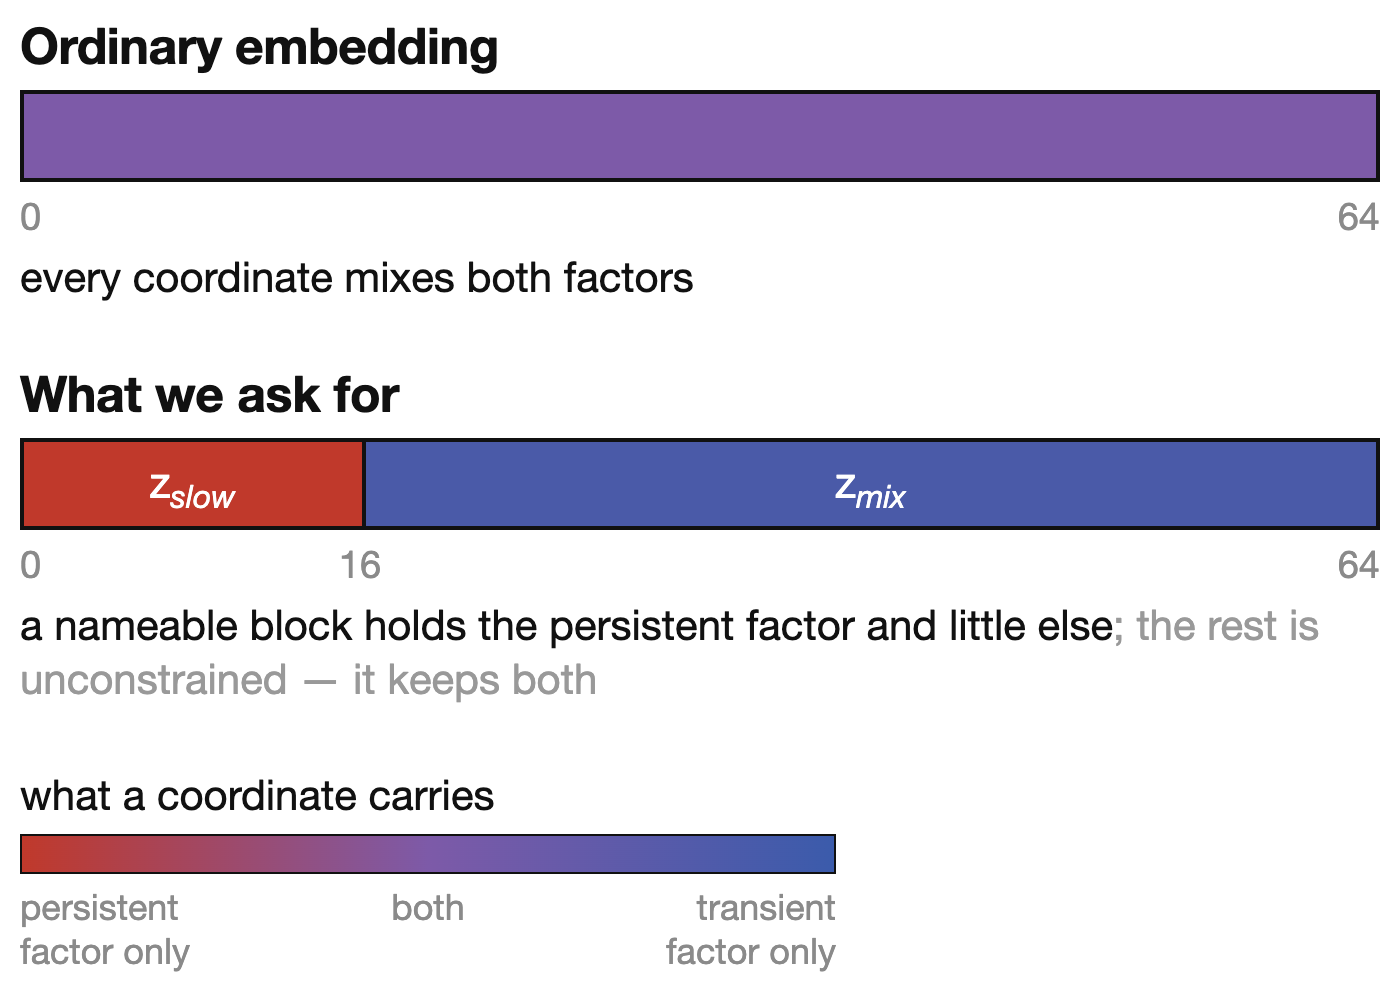
\includegraphics[width=0.9\textwidth]{figs/fig_concept_A.png}
\caption{\textbf{What we ask of the embedding.} In an ordinary embedding every one of the 64 coordinates mixes both factors. We ask instead that a nameable 16-dimensional block, $\zslow$, be emptied of the transient factor; the remaining block $\zmix$ is left unconstrained and keeps both. The claim is about what is \emph{absent} from $\zslow$, not about where the persistent factor can be found --- the latent space is rotation-symmetric, so any 16 coordinates carry it.}
\label{fig:concept}
\end{figure}

Our contributions are three. (i) An inductive bias that gates an already existing axis, the prediction horizon, splitting the persistent factor into a designatable block. (ii) An evaluation procedure that measures that separation with a block $\times$ factor matrix rather than from one side only, together with a single summarizing index, SEP. (iii) Measurements on synthetic data, PTB-XL, and HAPT. The results cut both ways. On synthetic data designed so that persistence and slowness disagree, we lead label-free post-hoc rotation on both stems (SEP 0.849 against SFA 0.388); on real data we trail SFA, which leads in three of four settings by margins of 0.032 to 0.072. We read this as a consequence of the relation between persistence and slowness --- on real data the two mostly coincide, so optimizing slowness directly does the same job more directly --- though we did not measure that causal link. Separation also carries a downstream cost (macro-F1 $-0.111$ on HAPT), which we quantify.
